\section{Introduction}
\label{sec:introduction}

Unit tests are an important artifact that supports the software development process in several ways.
%
In addition to helping developers ensure the quality of their software by checking for failures~\cite{daka2014survey}, they can also serve as an important source of documentation not only for human developers but also for automated software engineering tools (e.g., recent work on fault localization by \citeauthor{li2019deepfl} uses test name information~\cite{li2019deepfl}).
%
For example, when a test fails, its name can provide the first step towards understanding the purpose of the test and ultimately fixing the cause of the observed failure.
%
Similarly, a test's name can help developers decide whether a test should be left alone, modified, or removed in response to changes in the application under test and whether the test should be included in a regression test suite.


In this proposal, we believe that test names are \enquote{good} if they are descriptive (e.g, they accurately summarize both the scenario and the expected outcome of the test~\cite{trenk14}) and \enquote{bad} if they are not descriptive.
%
This is because descriptive names:
\begin{enumerate*}
\item make it easier to tell if some functionality is not being tested---if a behavior is not mentioned in the name of a test, then the behavior is not being tested
\item help prevent tests that are too large or contain unrelated assertions---if a test cannot be summarized, it likely should be split into multiple tests
\item serve as documentation for the class under test---a class's supported functionality can be identified by reading the names of its tests
\end{enumerate*}~\cite{zhang2015automatically}.


Unfortunately, unit tests often lack descriptive names~\cite{zhang2015automatically, daka2017generating}.
%
For example, an exploratory study by \citeauthor{zhang2015automatically} found that only \SI{9}{\percent} of the \num{213423} test names they considered were complete (i.e., fully described the body of test) while \SI{62}{\percent} were missing some information and \SI{29}{\percent} contained no useful information (e.g., tests named \enquote{test})~\cite{zhang2015automatically}.
%
Poor test names can be due to developers writing non-descriptive or incomplete names.
%
They can also occur due to incomplete code modifications.
%
For example, a developer may modify a test's body but fail to make the corresponding changes to the test's name.
%
Regardless of the cause, non-descriptive test names complicate comprehension tasks and increase the costs and difficulty of software development.


Because non-descriptive names negatively impact software development, there have been several attempts to address this issue. % POOR TEST NAMES
% Unit testing
For example, \citeauthor{zhang2016towards} and \citeauthor{daka2017generating} use static and dynamic analysis, respectively, to extract important expressions from a test's body and natural language processing techniques to transform such expression into test names \cite{zhang2016towards, daka2017generating}.
%
% TODO: Is there other work that goes here?

% Why this isnt good enough (i.e., doesn`t meet developer approval, does follow conventions, ... ')


% More general
More broadly, there have been attempts to to improve names for general identifiers and methods.
%
For example, \citeauthor{host2009debugging} proposed an approach for Java methods and variables which uses a set of naming rules and related semantics~\cite{host2009debugging}, and \citeauthor{li2019deepfl} provided a learning-based approach to locate software faults using test name information~\cite{li2019deepfl}.
%
Moreover, \citeauthor{allamanis2015suggesting} and \citeauthor{pradel2018deepbugs} used a model-based and a learning-based approach, respectively, to directly suggest better names or find name-based bugs to facilitate improvements~\cite{allamanis2015suggesting, pradel2018deepbugs}.
%
More recent work attempts to generate names that more closely match existing names by using machine learning to create approach that can map method bodies to method names (e.g.,~\cite{alon2018code2seq, alon2019code2vec}).
%
However, the success of these approaches heavily depend on their training sets and they are not always successful at creating models that match well with human cognition~\cite{lison2015introduction}.
%
In addition, these approaches are primarily geared towards general methods and have problems when applied to generating descriptive names for tests.
%
For example, we have found that, due to the similarity of test bodies, these approaches often generate duplicate names for tests in the same class (see~\cite{CodeResult}).
%
While such names make sense individually, they are useless in practice as duplicate names are not possible and, even if they were, they would not serve the goal of helping developers comprehend the purposes of their tests.


\begin{figure}[t]
\centering
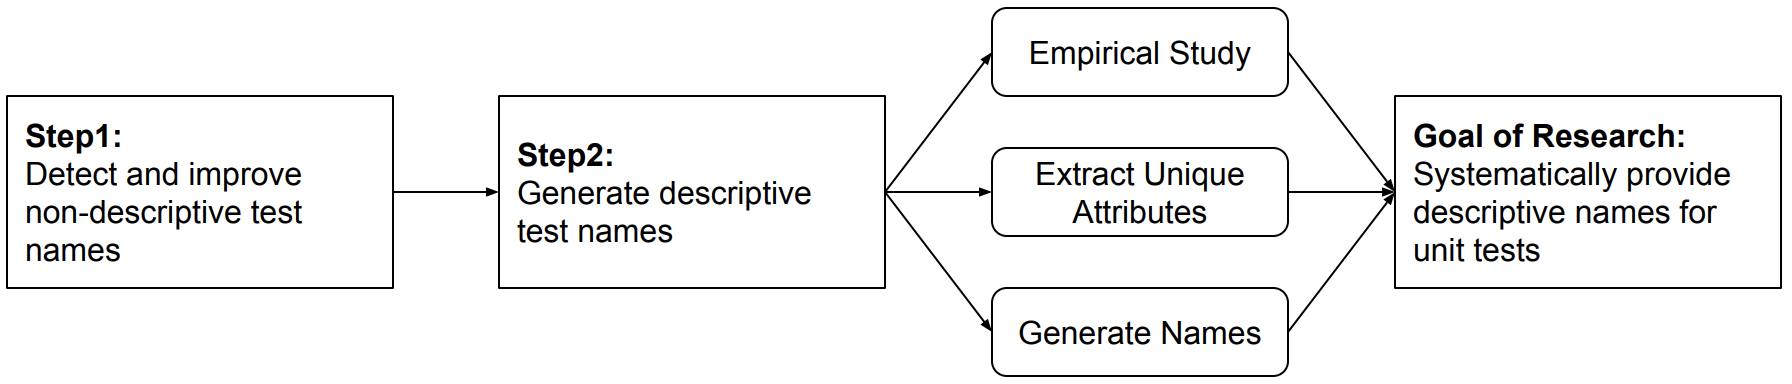
\includegraphics[scale=0.35]{figures/all-research.png}
\caption{Overview of research.}
\label{fig:all-research}
\end{figure}

The goal of my disseration work is to develop a set of approaches that can address the problem of poor, non-desecriptive test names.
%
At a high-level my work is divided into two pieces.


The first piece is to develop an apppraoch to detected non-describ names and, if possible, suggest improvments.
%
The approach is based on ....
\begin{enumerate*}
\item detect non-descriptive test names by finding information mismatches between the test name and body of a given JUnit test and provide descriptive information that is a summarization of the action, predicate, and scenario of the test body
\item use the descriptive information to facilitate the improvement of non-descriptive test names
\end{enumerate*}~\cite{wu2020pattern}.
%
Unlike existing approaches which were designed to handle general methods, our approach is specific to JUnit tests.
%
The narrower scope of allows the approach to take advantage of the highly repetitive structures that exist in both test names and bodies of JUnit tests (see~\cref{sec:test-pattern-section}).
%
From a high-level point of view, the pattern-based approach uses a set of predefined patterns to extract descriptive information from both a test's name and body.
%
This information is then compared to find and improve non-descriptive names (i.e., cases where the name does not accurately summarize the body).


The second piece, is to develop an approach to generate descriptive test names.
% % TODO What is the study of?
This piece contains three components.
The first component is an empirical study of naming rationales that investigates whether test are named after what makes them unique.
%
The results of the study
\begin{enumerate*}
\item confirm our impression that the majority of tests are named after what makes them unique
\item identify additional aspects that influence how tests are named
\end{enumerate*}.
%
The second component is a an automated approach for extracting the unique attributes of tests.
% TODO Describe second component.
The approach is encodes the knowledle gained from the study into a tool that uses selective codes, static analysis, and formal concept analysis (FCA) to identify unique attributes that agree with human judgment.


The final component will be a new approach for generating descriptive names based primarly on the unique attributes identify by the tool created in the second component.
%
Transforming the indentified attributes into a name is a nontrivial task... why?


% For the last sub-step\slash my planned future work, I plan to look into the majority of tests that were categorized as partially named after what makes the test unique.
% %
% Moreover, I will consider those minor naming rationales that were discovered in~\cref{sec:emp-study} and combine them with the uniqueness-based naming rationale that is widely adopted by developer.
% %
% The goal of these two investigations is to construct a comprehensive naming rationale that can cover as many existing tests as possible.
% %
% It will be based the uniqueness-based naming rationale but adequately enhanced to provide extensive information that help me construct descriptive test names.
% %
% I plan to build a descriptive name-generation approach that incorporates the formalized comprehensive naming rationale.
% %
% Based on the descriptive information provided by the formalized naming rationale, the generated names of the approach contain both the unique attributes and the essential information from other source or minor naming rationales.
% %
% Therefore, it would complete the second step of my dissertation work, which is to systemically provide descriptive names that meets with developer approval for unit tests.
% %
% I also plan to perform an empirical evaluation of the approach to check its performance (i.e., coverage, accuracy, and consistency).
